\begin{enunciado}
 Se lanza 180 veces un dado con los siguientes resultados:
 \begin{center}
  \begin{tabular}{c|cccccc}
   $x$ &  $1$ &  $2$ &  $3$ &  $4$ &  $5$ &  $6$ \\
   \hline
   $f$ & $28$ & $36$ & $36$ & $30$ & $27$ & $23$ 
  \end{tabular}
 \end{center}
 ¿Es un dado balanceado? Utilice un nivel de significancia de $0.01$.
\end{enunciado}

\begin{solucion}
 \begin{datos}
  $\phantom{0}$
  \begin{itemize}
   \item Tama\~no de la muestra: $n=180$.
   \item Frecuencias observadas:
   $O = (o_1 = 28, o_2 = 36, o_3 = 36, o_4 = 30, o_5 = 27, o_6 = 23)$.
   \item Probabilidades esperadas: $p_i = f(i;6)$,
   la funci\'on de probabilidad uniforme discreta con par\'ametro $k=6$,
   es decir $p_i = \frac{1}{6}, \forall i \in \mathbb{N}\cap[1,6]$.
   \item frecuencias esperadas:
   $E = \left\{ \left. e_i = n\cdot p_i = \frac{180}{6} = 30 \, \right| \, \forall i \in \mathbb{N}\cap[1,6] \right\}$.
   \item Celdas totales del experimento: $k=6$.
   \item Grados de libertad de la prueba $\chi^2$: $v = k-1 = 5$.
  \end{itemize}
 \end{datos}
 
 \begin{hipotesis}
  Prueba de bondad de ajuste para probar $H_0:$
  que una variable aleatoria $X$ sigue una distribuci\'on uniforme
  $f(x;k) = f(x;6)$, para $x \in\{1,2,3,4,5,6\}$
  contra la alternativa $H_1$ de que no es as\'{\i}.
 \end{hipotesis}

 \begin{significancia}
  $\alpha = 0.01$.
 \end{significancia}

 \begin{region}
  De la tabla A.5 se tiene el valor cr\'{\i}tico
  $\chi^2_{\alpha,v} = \chi^2_{0.01,5} = 15.086$,
  por lo que la regi\'on de rechazo est\'a dado
  para $\chi^2 > 15.086$, donde
  $\chi^2 = \sum_{i=1}^k \frac{\left( o_i - e_i \right)^2}{e_i}$.
 \end{region}

 \begin{estadistico}
  \begin{eqnarray*}
   \chi^2 & = & \sum_{i=1}^k \frac{\left( o_i - e_i \right)^2}{e_i} \\
   & = & \frac{(28 - 30)^2}{30} + \frac{(36-30)^2}{30} + \frac{(36 - 30)^2}{30}
   + \frac{(30 - 30)^2}{30} + \frac{(27-30)^2}{30} + \frac{(23 - 30)^2}{30} \\
   & = & \frac{4 + 36 + 36 + 0 + 9 + 49}{30} = \frac{134}{30}
   = \frac{67}{15} = 4.4\bar{6}
  \end{eqnarray*}
 \end{estadistico}

 \begin{decision}
  No se rechaza $H_0$.
 \end{decision}

 \begin{conclusion}
  No hay suficiente evidencia de que el dado no est\'a balanceado.
 \end{conclusion}

 En el c\'odigo registrado en el archivo \texttt{P15\_Prueba\_de\_bondad\_chi2\_01.r}, en R,
 se realiza este procedimiento.
 El c\'odigo permite modificar los valores iniciales que corresponden a:
 \texttt{datos} que guarda los datos de la lectura de un archivo,
 en este caso se lee el archivo \texttt{DB15\_Problema\_079.csv},
 y este \'ultimo nombre es el que se modifica para leer otros archivos;
 \texttt{varInteres} para indicar el nombre de la columna que corresponde a los datos en la base anterior;
 \texttt{varCelda} para indicar el nombre de la columna que corresponde
 a los datos de forma \'unica cuando ha sido agrupado en celdas,
 y, en este caso, la columna \texttt{varInteres} pasa a indicar
 las frecuencias de los valores, y si no hay agrupaci\'on de datos, 
 se asigna \texttt{NULL} a esta variable;
 \texttt{distribucion} indica, seg\'un una lista de valores,
 la distribuci\'on contra la que se va a comparar las observaciones,
 siendo la lista la siguiente: \texttt{1} para una uniforme discreta,
 \texttt{2} para una binomial, \texttt{3} para una hipergeom\'etrica y
 \texttt{4} para una geom\'etrica;
 en caso de que la distribuci\'on lleve par\'ametros supuestos,
 se indican el nombre y valor de cada uno de estos par\'ametros
 en las variables \texttt{parametro\_nombre} y \texttt{parametro\_valor},
 respectivamente;
 \texttt{combinar} para indicar, con \texttt{TRUE},
 que, si la frecuencia esperada en alguna celda es menor a $5$,
 se combinen celdas, y aunque se puede indicar con \texttt{FALSE}
 que no se realice este proceso, el no realizarlo puede dar
 un error, por lo que es recomendable mantenerlo;
 \texttt{grafica} para indicar, con \texttt{TRUE}, que se realizar\'a
 una gr\'afica comparando las proporciones observadas
 de las probabilidades esperadas,
 o \texttt{FALSE} en caso de no graficar;
 \texttt{tituloEjeX} para indicar el t\'{\i}tulo en el eje X
 cuando se realice una gr\'afica;
 y, \texttt{alfa} para el nivel de significancia.
 \par 
 El programa espera al menos los datos correspondientes a la base
 de datos, escrito en un archivo \texttt{.csv} con una columna
 con todos los datos, o una agrupaci\'on de los datos con sus frecuencias, 
 y la distribuci\'on con la que se va a comparar los datos.
 \par 
 El programa permite agregar par\'ametros junto con la distribuci\'on
 de ajuste, seg\'un el tipo de distribuci\'on:
 para la distribuci\'on uniforme discreta no se requieren par\'ametros;
 para la distribuci\'on binomial puede llevar el par\'ametro $p$
 correspondiente a la probabilidad de \'exito;
 para la distribuci\'on hipergeom\'etrica pueden asignarse
 los par\'ametros $N$ para el tama\~no de poblaci\'on,
 $n$ para el tama\~no muestral y $k$ para la cantidad de casos favorables,
 sin embargo, aunque son opcionales, si se requiere
 que al menos uno de los 2 entre $N$ y $k$ sea asignado,
 ya que no se ha encontrado alg\'un m\'etodo para estimar ambos
 simult\'aneamente a partir de los datos;
 y, para la distribuci\'on geom\'etrica, se puede asignar $p$
 para la probabilidad de \'exito.
 Seg\'un la literatura acerca de la prueba de ajsute de bondad $\chi^2$,
 por cada par\'ametro que se estime, se debe reducir en 1
 la cantidad de grados de libertad,
 lo cual se ve reflejado en el programa.
 Adicional a esta nota, tambi\'en cabe mencionar que, para la gr\'afica,
 el programa de R requiere del paquete \texttt{MASS}.
 \par
 Independientemente de c\'omo se realice la prueba, 
 el resultado muestra lo siguiente:
 \texttt{Variable} que indica el nombre y unidad
 de lo que se est\'a midiendo;
 \texttt{Distribuci\'on de ajuste} que indica el nombre
 de la distribuci\'on con la que se est\'an comparando los datos;
 \texttt{Estad\'{\i}stico Chisq2} para el valor del estad\'{\i}stico
 $\chi^2$;
 \texttt{Grados de libertad} o \texttt{Grados de libertad ajustado}
 para indicar la cantidad de grados de libertad usando en los c\'alculos
 de probabilidades de la distribuci\'on $\chi^2$;
 \texttt{Valor-p} o \texttt{Valor-p ajustado} para indicar
 el $p-$valor, cuyo nombre depende respectivamente de si se supuso
 todos los par\'ametros o si se hizo alg\'un ajuste;
 \texttt{alpha} que muestra el valor asignado en la variable \texttt{alfa} \'o $0.05$ en caso de que se le haya asignado \texttt{NULL};
 \texttt{Regi\'on de rechazo} indicando a partir de cu\'al valor
 se rechaza el estad\'{\i}stico, seg\'un el valor \texttt{alpha} mostrado.
 \par
 Adem\'as, si se han indicado par\'ametros estpec\'{\i}ficos
 en la comparaci\'on del ajuste, estos se muestran a continuaci\'on
 de la distribuci\'on; y puede aparecer el valor de \texttt{Resultado}
 para indicar si se rechaza o no la hip\'otesis nula,
 que aparece al final de los resultados cuando se asigna un valor
 a \texttt{alpha}.
 \par 
 El c\'odigo junto con el resultado se muestra a continuaci\'on:
 \begin{verbatim}
> require(MASS)
> datos<-read.csv("DB15_Problema_079.csv",sep=";",encoding="UTF-8")
> varInteres<-"Frecuencia"
> varCelda<-"Lanzamiento.valor"
> distribucion<-1
> parametro_nombre<-NULL
> parametro_valor<-NULL
> combinar<-TRUE
> grafica<-TRUE
> tituloEjeX<-"Resultados al lanzar un dado"
> alfa<-0.01
> valores<-datos[,varInteres]
> valores<-valores[!is.na(valores)]
> if(is.null(varCelda)){
+   frecuencia<-as.vector(table(valores))
+   valores<-as.integer(names(table(valores)))
+ }else{
+   frecuencia<-valores[order(datos[,varCelda])]
+   valores<-sort(datos[,varCelda])
+   varInteres<-varCelda
+ }
> cantParametros<-min(length(parametro_nombre),length(parametro_valor))
> diccionario_parametros<-data.frame(Nombre=parametro_nombre[1:cantParametros],
+                                    Valor=parametro_valor[1:cantParametros])
> switch(distribucion,
+        nomDist<-"Uniforme",
+        nomDist<-"Binomial",
+        nomDist<-"Hipergeométrica",
+        nomDist<-"Geométrica")
> switch(distribucion,
+        maxParam<-0,
+        maxParam<-1,
+        maxParam<-3,
+        maxParam<-1)
> colapsar<-function(p1,f1,lim1=5){
+   np1<-p1
+   nf1<-f1
+   tocollapse<-which((np1*sum(nf1))<lim1)
+   while(length(tocollapse)>0){
+     x<-tocollapse[1]
+     if (x<length(np1)){
+       np1[x+1]<-p1[x]+p1[x+1]
+       nf1[x+1]<-f1[x]+f1[x+1]
+     }else{
+       np1[x-1]<-p1[x]+p1[x-1]
+       nf1[x-1]<-f1[x]+f1[x-1]
+     }
+     p1<-np1[-x]
+     f1<-nf1[-x]
+     np1<-p1
+     nf1<-f1
+     tocollapse<-which((p1*sum(f1))<lim1)
+   }
+   return(list(probs=p1,freqs=f1))  
+ }
> calculos<-function(valores,frecuencia,distribucion,parametros,alfa=0.05){
+   if(length(frecuencia)>1){
+     r<-NULL
+     if(distribucion==1){
+       k<-length(frecuencia)
+       frecObs<-frecuencia
+       probEsp<-rep(1/k,k)
+       if(combinar){
+         r1<-colapsar(probEsp,frecObs)
+         frecObsC<-r1$freqs
+         probEspC<-r1$probs
+         if(length(frecObsC)>1){
+           prueba<-chisq.test(frecObsC,p=probEspC)
+         }else{
+           prueba<-NA
+         }
+       }else{
+         prueba<-chisq.test(frecObs,p=probEsp)
+       }
+       if(!is.na(prueba[1]) & prueba$parameter > 0){
+         r<-c(prueba$statistic, prueba$parameter,prueba$p.value,alfa,
+              qchisq(alfa,prueba$parameter,lower.tail=FALSE))
+       }else{
+         r<-rep(NA,3)
+       }
+     }else if(distribucion==2){
+       ajustado<-identical(which(parametros$Nombre=="p"),integer(0))
+       n<-max(valores)
+       if(ajustado){
+         media<-sum(valores*frecuencia)/sum(frecuencia)
+         prob1<-media/n
+       }else{
+         prob1<-parametros$Valor[which(parametros$Nombre=="p")]
+       }
+       frecObs<-frecuencia
+       probEsp<-dbinom(0:n,size=n,prob=prob1)
+       if(combinar){
+         r1<-colapsar(probEsp,frecObs)
+         frecObsC<-r1$freqs
+         probEspC<-r1$probs
+         if(length(frecObsC)>1){
+           prueba<-chisq.test(frecObsC,p=probEspC)
+         }else{
+           prueba<-NA
+         }
+       }else{
+         prueba<-chisq.test(frecObs,p=probEsp)
+       }
+       if(!is.na(prueba[1]) & prueba$parameter > 0){
+         if(ajustado){
+           r<-c(prueba$statistic, prueba$parameter-1,
+                pchisq(prueba$statistic, prueba$parameter-1,lower.tail=FALSE),
+                alfa, qchisq(alfa,prueba$parameter-1,lower.tail=FALSE))
+         }else{
+           r<-c(prueba$statistic, prueba$parameter, prueba$p.value,alfa,
+                qchisq(alfa,prueba$parameter,lower.tail=FALSE))
+         }
+       }else{
+         r<-rep(NA,3)
+       }
+     }else if(distribucion==3){
+       estimarN<-identical(integer(0),which(parametros$Nombre=="N"))
+       estimarn<-identical(integer(0),which(parametros$Nombre=="n"))
+       estimark<-identical(integer(0),which(parametros$Nombre=="k"))
+       ajustes<-0
+       if(estimarn){
+         n<-max(valores)
+         ajustes<-ajustes+1
+       }else{
+         n<-parametros$Valor[which(parametros$Nombre=="n")]
+       }
+       if(!estimarN | !estimark){
+         if(estimark) {
+           N<-parametros$Valor[which(parametros$Nombre=="N")]
+           media<-sum(valores*frecuencia)/sum(frecuencia)
+           k<-round(media*N/n,0)
+           ajustes<-ajustes+1
+         }else{
+           k<-parametros$Valor[which(parametros$Nombre=="k")]
+           if(estimarN) {
+             media<-sum(valores*frecuencia)/sum(frecuencia)
+             N<-floor(n*k/media)
+             ajustes<-ajustes+1
+           }else{
+             N<-parametros$Valor[which(parametros$Nombre=="N")]
+           }
+         }
+       }else{
+         stop("No se puede estimar a la vez N y k.")
+       }
+       frecObs<-frecuencia
+       probEsp<-dhyper(0:n,k,N-k,n)
+       if(combinar){
+         r1<-colapsar(probEsp,frecObs)
+         frecObsC<-r1$freqs
+         probEspC<-r1$probs
+         if(length(frecObsC)>1){
+           prueba<-chisq.test(frecObsC,p=probEspC)
+         }else{
+           prueba<-NA
+         }
+       }else{
+         prueba<-chisq.test(frecObs,p=probEsp)
+       }
+       if(!is.na(prueba[1]) & prueba$parameter-ajustes> 0){
+         r<-c(prueba$statistic, prueba$parameter-ajustes,
+              pchisq(prueba$statistic, prueba$parameter-ajustes,
+                     lower.tail=FALSE),
+              alfa, qchisq(alfa,prueba$parameter-ajustes,lower.tail=FALSE))
+       }else{
+         r<-rep(NA,3)
+       }
+     }else if(distribucion==4){
+       ajustes<-as.integer(identical(which(parametros$Nombre=="p"),integer(0)))
+       n<-max(valores)
+       if(ajustes){
+         media<-sum(valores*frecuencia)/sum(frecuencia)
+         prob1<-1/media
+       }else{
+         prob1<-parametros$Valor[which(parametros$Nombre=="p")]
+       }
+       frecObs<-frecuencia
+       probEsp<-dgeom(0:(n-2),prob1)
+       probEsp<-c(probEsp, 1-sum(probEsp))
+       if(combinar){
+         r1<-colapsar(probEsp,frecObs)
+         frecObsC<-r1$freqs
+         probEspC<-r1$probs
+         if(length(frecObsC)>1){
+           prueba<-chisq.test(frecObsC,p=probEspC)
+         }else{
+           prueba<-NA
+         }
+       }else{
+         prueba<-chisq.test(frecObs,p=probEsp)
+       }
+       if(!is.na(prueba[1]) & prueba$parameter-ajustes> 0){
+         r<-c(prueba$statistic, prueba$parameter-ajustes,
+              pchisq(prueba$statistic, prueba$parameter-ajustes,
+                     lower.tail=FALSE),
+              alfa, qchisq(alfa,prueba$parameter-ajustes,lower.tail=FALSE))
+       }else{
+         r<-rep(NA,3)
+       }
+     }
+     if(is.null(r)){
+       r<-rep(NA,3)
+     }
+     return(r)
+   }
+ }
> if(!is.null(alfa)){
+   tabla<-t(as.matrix(calculos(valores,frecuencia,distribucion,
+                               diccionario_parametros,alfa)))
+ }else{
+   tabla<-t(as.matrix(calculos(valores,frecuencia,distribucion,
+                               diccionario_parametros)))
+ }
> if(cantParametros>0){
+   tabla<-data.frame(nombre=varInteres,Ajuste=nomDist,
+                     t(parametro_valor[1:cantParametros]),tabla)
+   auxNombresParam<-parametro_nombre
+ }else{
+   tabla<-data.frame(nombre=varInteres,Ajuste=nomDist,tabla)
+   auxNombresParam<-NULL
+ }
> if (cantParametros!=maxParam) {
+     names(tabla)<-c("Variable","Distribución de ajuste",auxNombresParam,
+                     "Estadístico Chisq2","Grados de libertad ajustado",
+                     "Valor-p ajustado","alpha","Región de Rechazo")
+ }else{
+   names(tabla)<-c("Variable","Distribución de ajuste",auxNombresParam,
+                   "Estadístico Chisq2","Grados de libertad",
+                   "Valor-p","alpha","Región de Rechazo")
+ }
> tabla["Región de Rechazo"]<-paste(">",round(tabla["Región de Rechazo"],7))
> generaGrafica<-function(valores,frecuencia,parametros=NULL,distribucion=1,
+                       tituloEjeX,nomVariable){
+   x<-c()
+   for(i in 1:length(valores)){
+     x<-c(x,rep(valores[i],frecuencia[i]))
+   }
+   maxD<-max(density(x)$y)
+   if(distribucion==1){
+     k<-max(x)-min(x)+1
+     probEspG<-rep(1/k,k+3)
+     x11()
+     truehist(x,h=1,
+              main=paste("Comparación de distribuciones","\n",nomDist),
+              xlab=tituloEjeX, ylab="Densidad",sub=nomVariable,
+              xlim=c((min(x)-1),(max(x)+2)),
+              ymax=max(max(probEspG),maxD)*1.2)
+     lines((min(x)-1):(max(x)+2),probEspG,type="s",col="red",lty=2,lwd=2)
+     legend("topleft",legend = c("Dist. original", "Dist. teórica"),
+            lwd=c(1,2),lty=2,col=c("black","red"))
+   }else if(distribucion==2){
+     n<-max(valores)
+     if(identical(which(parametros$Nombre=="p"),integer(0))){
+       media<-sum(valores*frecuencia)/sum(frecuencia)
+       prob1<-media/n
+     }else{
+       prob1<-parametros$Valor[which(parametros$Nombre=="p")]
+     }
+     probEspG<-dbinom(0:(max(x)+1),size=n,prob=prob1)
+     x11()
+     truehist(x,h=1,main=paste("Comparación de distribuciones","\n",nomDist),
+              xlab=tituloEjeX,ylab="Densidad",sub=nomVariable,
+              xlim=c((min(x)-1),(max(valores)+2)),
+              ymax=max(max(probEspG),maxD)*1.2)
+     lines(0:(max(x)+2),c(probEspG,0),type="s",col="red",lty=2,lwd=2)
+     legend("topleft",legend=c("Dist. original","Dist. teórica"),
+            lwd=c(1,2),lty=2,col=c("black","red"))
+   }else if(distribucion==3){
+     estimarN<-identical(integer(0),which(parametros$Nombre=="N"))
+     estimarn<-identical(integer(0),which(parametros$Nombre=="n"))
+     estimark<-identical(integer(0),which(parametros$Nombre=="k"))
+     if(estimarn){
+       n<-max(valores)
+     }else{
+       n<-parametros$Valor[which(parametros$Nombre=="n")]
+     }
+     if(!estimarN | !estimark){
+       if(estimark) {
+         N<-parametros$Valor[which(parametros$Nombre=="N")]
+         media<-sum(valores*frecuencia)/sum(frecuencia)
+         k<-round(media*N/n,0)
+       }else{
+         k<-parametros$Valor[which(parametros$Nombre=="k")]
+         if(estimarN) {
+           media<-sum(valores*frecuencia)/sum(frecuencia)
+           N<-floor(n*k/media)
+         }else{
+           N<-parametros$Valor[which(parametros$Nombre=="N")]
+         }
+       }
+     }
+     probEspG<-dhyper(0:(n+1),k,N-k,n)
+     x11()
+     truehist(x,h=1,main=paste("Comparación de distribuciones","\n",nomDist),
+              xlab=tituloEjeX,ylab="Densidad",sub=nomVariable,
+              xlim=c((min(x)-1),(max(valores)+2)),
+              ymax=max(max(probEspG),maxD)*1.2)
+     lines(0:(max(x)+2),c(probEspG,0),type="s",col="red",lty=2,lwd=2)
+     legend("topleft",legend=c("Dist. original","Dist. teórica"),
+            lwd=c(1,2),lty=2,col=c("black","red"))
+   }else if(distribucion==4){
+     ajustes<-as.integer(identical(which(parametros$Nombre=="p"),integer(0)))
+     n<-max(valores)
+     if(ajustes){
+       media<-sum(valores*frecuencia)/sum(frecuencia)
+       prob1<-1/media
+     }else{
+       prob1<-parametros$Valor[which(parametros$Nombre=="p")]
+     }
+     probEspG<-dgeom(0:(n-2),prob1)
+     probEspG<-c(probEspG, 1-sum(probEspG))
+     x11()
+     truehist(x,h=1,main=paste("Comparación de distribuciones","\n",nomDist),
+              xlab=tituloEjeX,ylab="Densidad",sub=nomVariable,
+              xlim=c((min(x)-1),(max(valores)+2)),
+              ymax=max(max(probEspG),maxD)*1.2)
+     lines(1:(max(x)+1),c(probEspG,0),type="s",col="red",lty=2,lwd=2)
+     legend("topleft",legend=c("Dist. original","Dist. teórica"),
+            lwd=c(1,2),lty=2,col=c("black","red"))
+   }
+   invisible()
+ }
> if(!is.null(alfa)){
+   tabla$alpha<-alfa
+   tabla$Resultado<-ifelse(tabla$"Valor-p">=alfa,
+                          "No se rechaza el ajuste de bondad",
+                          "Se rechaza el ajuste de bondad")
+ }
> tabla
           Variable Distribución de ajuste Estadístico Chisq2 Grados de libertad
1 Lanzamiento.valor               Uniforme           4.466667                  5
    Valor-p alpha Región de Rechazo                         Resultado
1 0.4843557  0.01      > 15.0862725 No se rechaza el ajuste de bondad
> if (grafica){
+   generaGrafica(valores,frecuencia,diccionario_parametros,
+                 distribucion,tituloEjeX,varInteres)
+ }
 \end{verbatim}
 \vspace{-0.5cm}
 que incluye la siguiente figura:
 \begin{center}
  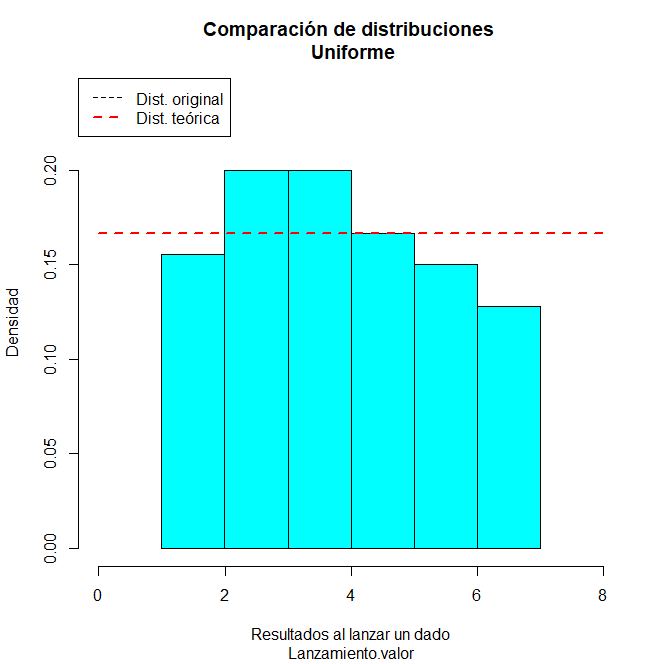
\includegraphics[scale=0.35]{Problema_79.png}
 \end{center}
 El cual coincide con los resultados obtenidos,
 adem\'as de ofrecer informaci\'on como el valor $P$,
 que es a lo que se quer\'{\i}a llegar.${}_{\blacksquare}$
\end{solucion}
